\newpage

%%%%%%%%%%%%%%%%%%%%%%%%%%%%%%%%%%%%%%%%%%%%%%%%%%%%%%%%%%%%%%%%%%%%%%%%%%%%%%%%%%%%%%%
%%%%%%%%%%%%%%%%%%%%%%%%%%%%%%%%%%%%%%%%%%%%%%%%%%%%%%%%%%%%%%%%%%%%%%%%%%%%%%%%%%%%%%%
%%%%%%%%%%%%%%%%%%%%%%%%%%%%%%%%%%%%%%%%%%%%%%%%%%%%%%%%%%%%%%%%%%%%%%%%%%%%%%%%%%%%%%%
\section{Regressão logística-não linear e SE com classificador $f_{\VECTOR{c}}(\VECTOR{x}):~\mathbb{R}^{N} \rightarrow \mathbb{R}$}
\label{sec:theo:reglogrnr1nolinear:1}

\index{Regressão!Logística polinomial $f_{\VECTOR{c}}(\VECTOR{x}):~\mathbb{R}^{N} \rightarrow \mathbb{R}$}
\index{Polinômio multivariante}

\begin{theorem}[Classificação de dados em $\mathbb{R}^{N}$:]\label{theo:reglogrnr1nolinear:1}
~\\
\noindent
\begin{minipage}{0.45\textwidth}
\centering
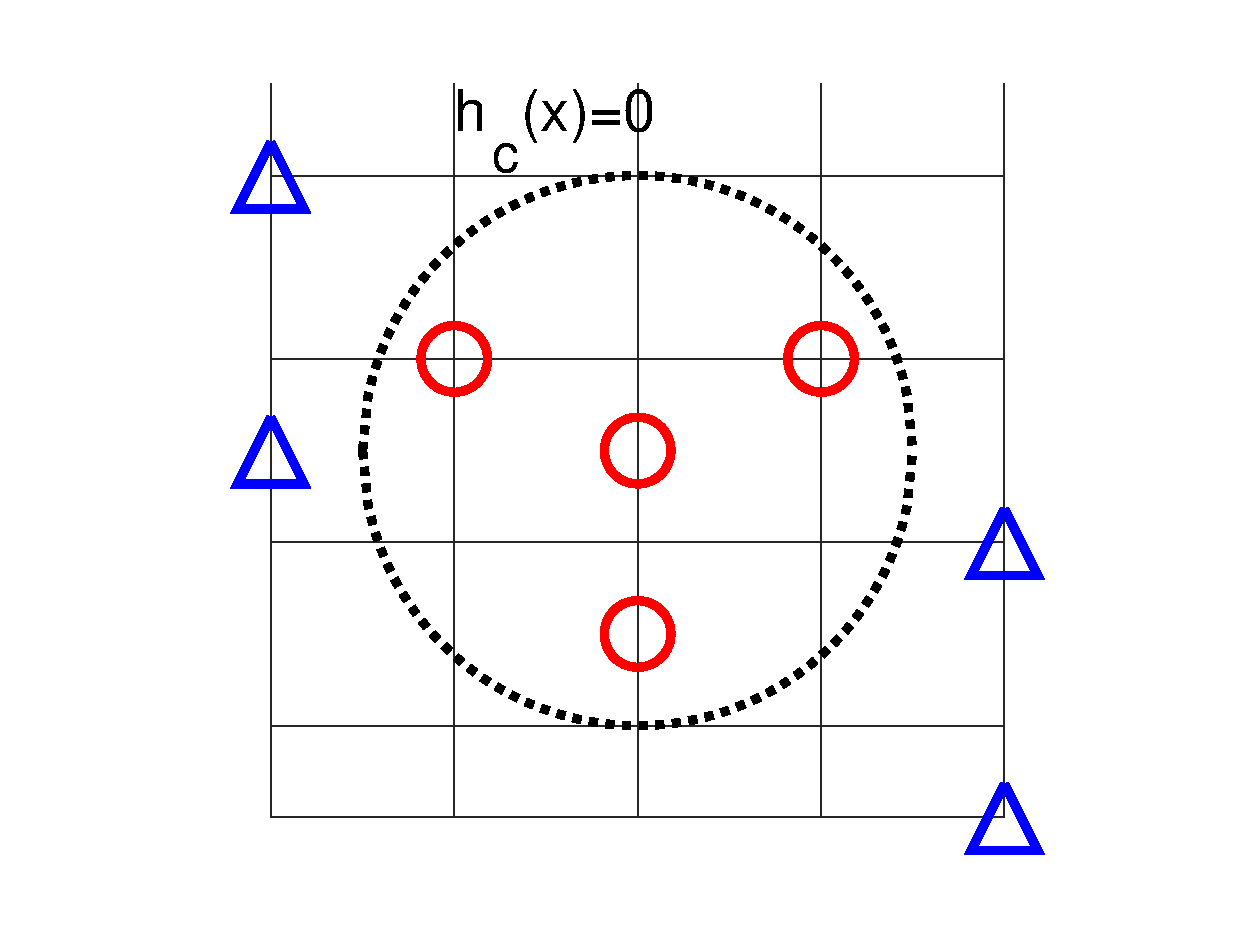
\includegraphics[width=0.95\linewidth]{chapters/classificacao/mfiles/reglogrnr1nolinear/reglogrnr1nolinear.eps} 
\end{minipage}
\begin{minipage}{0.55\textwidth}
Dados, um conjunto de $L$ pontos
$\VECTOR{x}_l$ $\in \mathbb{R}^{N}$, $1\leq l \leq L$,
repartidos em dois grupos etiquetados com os símbolos $\bigtriangleup$ e $\bigcirc$,
não separáveis por um hiperplano  em $\mathbb{R}^{N}$.
Se desejamos criar um classificador mediante 
a função  $f_{\VECTOR{c}}:\mathbb{R}^{N} \rightarrow \mathbb{R}$,
com domínio $\VECTOR{x} \in \mathbb{R}^{N}$, contradomínio $y \in \mathbb{R}$ e 
parâmetros agrupados no vetor $\VECTOR{c} \in \mathbb{R}^{M}$,
como definido na Eq. (\ref{eq:reglogrnr1nolinear:1}),
\begin{equation}\label{eq:reglogrnr1nolinear:1}
y\equiv f_{\VECTOR{c}}(\VECTOR{x})= \frac{1}{1+e^{-h_{\VECTOR{c}}(\VECTOR{x})}},
\end{equation}
\end{minipage}
ou seu equivalente, $logit(y)=h_{\VECTOR{c}}(\VECTOR{x})\equiv h(\VECTOR{c},\VECTOR{x})$,
onde $h_{\VECTOR{c}}: \mathbb{R}^{N} \rightarrow \mathbb{R}$ é uma função não linear
com domínio $\VECTOR{x}$ e
com coeficientes $\VECTOR{c}=[c_1,~c_2,~...,~c_M]^{\transpose}$.
Podemos atribuir a cada ponto $\VECTOR{x}_l$ uma etiqueta $y_l\in \{A,1-A\}$, 
$A$ para $\bigtriangleup$ e  $1-A$ para $\bigcirc$,
onde $0<A\ll 0.5$ é escolhido por nós,
e afirmar que o vetor $\VECTOR{c}= \VECTOR{\hat{c}}$,
que minimiza o erro quadrático $e(\VECTOR{c})$,
\begin{equation}\label{eq:reglogrnr1nolinear:1e}
e(\VECTOR{c}) =  ||\VECTOR{h}(\VECTOR{c})-\VECTOR{z}||_{\MATRIX{W}}^2 + \alpha||\VECTOR{c}-\VECTOR{c}_{last}||_{\MATRIX{D}}^2,
\end{equation}
\begin{equation}
\VECTOR{h}(\VECTOR{c})=\begin{bmatrix}
h_{\VECTOR{c}}(\VECTOR{x}_1)\\ 
h_{\VECTOR{c}}(\VECTOR{x}_2)\\ 
%\vdots\\ 
%h_{\VECTOR{c}}(\VECTOR{x}_l)\\ 
\vdots\\ 
h_{\VECTOR{c}}(\VECTOR{x}_L)
\end{bmatrix},
~
%\MATRIX{P}=\begin{bmatrix}
%\VECTOR{x}_1^{\transpose}\\ 
%\VECTOR{x}_2^{\transpose}\\ 
%%\vdots\\ 
%%\VECTOR{x}_l^{\transpose}\\ 
%\vdots\\ 
%\VECTOR{x}_L^{\transpose}
%\end{bmatrix},
%~
\VECTOR{z}=
\begin{bmatrix}
logit(y_1)  \\
logit(y_2)  \\
%\vdots  \\
%logit(y_l)  \\
\vdots \\
logit(y_L) \\
\end{bmatrix},
~
\MATRIX{W}=\funcdiag\left(\begin{bmatrix}
w_1\\ 
w_2\\ 
%\vdots\\ 
%w_l\\ 
\vdots\\ 
w_L
\end{bmatrix}\right),
~
\MATRIX{D}=\funcdiag\left(\begin{bmatrix}
d_1\\ 
d_2\\ 
%\vdots\\ 
%d_m\\ 
\vdots\\ 
d_M
\end{bmatrix}\right),
\end{equation}
pode ser achado\footnote{A demostração pode ser vista na Prova \ref{proof:theo:reglogrnr1nolinear}.} 
usando de forma iterativa a Eq. (\ref{eq:reglogrnr1nolinear:2}),
sendo que $w_l \in \mathbb{R}_+$, $d_l \in \mathbb{R}_+$, e $\alpha \in \mathbb{R}_+$ são valores escolhido por nós;
\begin{equation}\label{eq:reglogrnr1nolinear:2}
\VECTOR{c}_{i}=\VECTOR{c}_{i-1}-[\MATRIX{J}(\VECTOR{c}_{i-1})^{\transpose}\MATRIX{W}\MATRIX{J}(\VECTOR{c}_{i-1})+\alpha \MATRIX{D}]^{-1}\MATRIX{J}(\VECTOR{c}_{i-1})^{\transpose}\MATRIX{W}[\VECTOR{h}(\VECTOR{c}_{i-1})-\VECTOR{z}],
\end{equation}
onde a matriz $\MATRIX{J}(\VECTOR{c})$ 
$\equiv \frac{\partial \VECTOR{h}(\VECTOR{c})}{\partial \VECTOR{c}^{\transpose}}$ é a 
\hyperref[def:jacobian]{\textbf{matriz Jacobiana}}  de $\VECTOR{h}(\VECTOR{c})$,
\begin{equation}\label{eq:reglogrnr1nolinear:3}
\MATRIX{J}(\VECTOR{c})=\begin{bmatrix}
\VECTOR{j}(\VECTOR{c},\VECTOR{x}_1)\\ 
\VECTOR{j}(\VECTOR{c},\VECTOR{x}_2)\\ 
%\vdots\\ 
%\VECTOR{j}(\VECTOR{c},\VECTOR{x}_l)\\ 
\vdots\\ 
\VECTOR{j}(\VECTOR{c},\VECTOR{x}_L)
\end{bmatrix},
\quad
\begin{array}{lll}
\VECTOR{j}(\VECTOR{c},\VECTOR{x}) & = & \frac{\partial h(\VECTOR{c},\VECTOR{x})}{\partial \VECTOR{c}^{\transpose}} \\
                       ~ & ~ & ~\\
                       ~ & = & \left[\frac{\partial h(\VECTOR{c},\VECTOR{x})}{\partial c_1}\quad \frac{\partial h(\VECTOR{c},\VECTOR{x})}{\partial c_2}\quad  ... \quad \frac{\partial h(\VECTOR{c},\VECTOR{x})}{\partial c_{M}} \right].
\end{array}
\end{equation}

\textbf{Considerações:}
\begin{itemize}
\item A busca iterativa da Eq. (\ref{eq:reglogrnr1nolinear:2}) 
é declarada finalizada com sucesso 
quando iterações consecutivas do vetor $\VECTOR{c}_i$ convergem a valores próximos, onde declaramos $\VECTOR{\hat{c}}=\VECTOR{c}_i$.
\item O erro mínimo, $e(\VECTOR{\hat{c}}) \geq 0$, não necessariamente ter valor zero. 
\end{itemize}
\end{theorem}
~

\begin{tcbattention}
\begin{itemize}
\item Dado que a função de classificação $f_{\VECTOR{c}}(\VECTOR{x})$ vai entre $0$ e $1$,
podemos reinterpretar este valor como se fosse uma probabilidade;
neste caso, $f_{\VECTOR{c}}(\VECTOR{x})$ representa a probabilidade de que um ponto $\VECTOR{x}$
pertença ao grupo $\bigcirc$.
\item O limiar de classificação na função $f_{\VECTOR{c}}(\VECTOR{x})$ está na superfície $h_{\VECTOR{c}}(\VECTOR{x})=0$,
provocando nestos pontos um $f_{\VECTOR{c}}(\VECTOR{x})=0.5$.
\end{itemize}
\end{tcbattention}

%%%%%%%%%%%%%%%%%%%%%%%%%%%%%%%%%%%%%%%%%%%%%%%%%%%%%%%%%%%%%%%%%%%%%%%%%%%%%%%%
\subsection{Exemplos de classificação com uma função
$f_{\VECTOR{c}}(\VECTOR{x}):~\mathbb{R}^N \rightarrow \mathbb{R}$ }

\begin{example}\label{ex:theo:reglogrnr1nolinear}
Conhecidas as $L=10$ amostras $\VECTOR{x}_l$ e seus respetivos grupos indicados pelos símbolos $\bigtriangleup$ e $\bigcirc$, 
mostrados na Tabela \ref{table:theo:reglogrnr1nolinear:xn},
achar o classificador $f_{\VECTOR{c}}(\VECTOR{x})$ que usa a função 
$h_{\VECTOR{c}}(\VECTOR{x})=c_1\left( \left(x_1-c_2\right)^2 + \left(x_2-c_3\right)^2 -c_4^2\right)$, 
que gere o menor erro $e(\VECTOR{c}) =  ||\VECTOR{h}(\VECTOR{c})-\VECTOR{z}||^2$ $+$ $0.001~||\VECTOR{c}-\VECTOR{c}_{last}||^2$.
\end{example}


\begin{table}[h!]
\centering
\begin{tabular}{|c||c|c|c|c|c||c|c|c|c|c||} 
 \hline
$l$            & 1 & 2 & 3 & 4 & 5 & 6 & 7 & 8 & 9 & 10 \\ \hline \hline
$\VECTOR{x}_l$ & 6 & 2 & 2 & 6 & 6 & 4 & 3 & 3 & 4 & 4 \\ 
~              & 5 & 5 & 1 & 1 & 3 & 4 & 4 & 3 & 2 & 3 \\ \hline
$\VECTOR{y}_l$ & $\bigtriangleup$ & $\bigtriangleup$ & $\bigtriangleup$ & $\bigtriangleup$ & $\bigtriangleup$ 
      & $\bigcirc$ & $\bigcirc$ & $\bigcirc$ & $\bigcirc$ & $\bigcirc$\\ \hline
\end{tabular}
\caption{Pontos $\VECTOR{x}_l$.}
\label{table:theo:reglogrnr1nolinear:xn}
\end{table}


\begin{SolutionT}[Relativa ao Exemplo \ref{ex:theo:reglogrnr1nolinear}:]\label{sol:theo:reglogrnr1nolinear:s1}
Para obter o vetor de parâmetros $\VECTOR{c}=\VECTOR{\hat{c}}$ da função $f_{\VECTOR{c}}(\VECTOR{x})$, 
que gere o menor erro $e(\VECTOR{c})$
com os $L=10$ dados $\VECTOR{x}_l$ da Tabela \ref{table:theo:reglogrnr1nolinear:xn},
usamos a Eq. (\ref{eq:reglogrnr1nolinear:2}) onde escolhemos $\alpha=0.001$, $d_l=w_l=1$ e valores $y_l \in \{0.001,~ 0.999\}$,
$0.001$ para $\bigtriangleup$ e $0.999$ para $\bigcirc$;
além disso calculamos 
\begin{equation}
\VECTOR{j}(\VECTOR{c},\VECTOR{x}) = 
\left[ 
\left(x_1-c_2\right)^2 + \left(x_2-c_3\right)^2 -c_4^2, \quad 
-2c_1\left(x_1-c_2\right), \quad
-2c_1\left(x_2-c_3\right), \quad
-2c_1c_4
\right],
\end{equation}
obtendo um vetor $\VECTOR{\hat{c}}=[-1.8915,~ 3.7830,~ 3.0296,~ -2.0352]^{\transpose}$.
Assim, a função $\left.f_{\VECTOR{c}}(x)\right|_{\VECTOR{c}=\VECTOR{\hat{c}}}$ que classifica os dados $\VECTOR{x}_l$
é mostrada na Eq. (\ref{eq:theo:reglogrnr1nolinear:xn:s1}) e na Figura \ref{fig:theo:reglogrnr1nolinear:xn:s1},
\begin{equation}\label{eq:theo:reglogrnr1nolinear:xn:s1}
f_{\VECTOR{\hat{c}}}(\VECTOR{x})= \frac{1}{1+e^{-h_{\VECTOR{\hat{c}}}(\VECTOR{x})}},
\quad
h_{\VECTOR{\hat{c}}}(\VECTOR{x}) = -1.8915\left( \left(x_1-3.7830\right)^2 + \left(x_2-3.0296\right)^2 -2.0352^2\right).\\
\end{equation}
É interessante ressaltar que o limiar de classificação está na superfície $h_{\VECTOR{\hat{c}}}(\VECTOR{x})=0$.
\end{SolutionT}
\begin{figure}[!h]
        \centering
        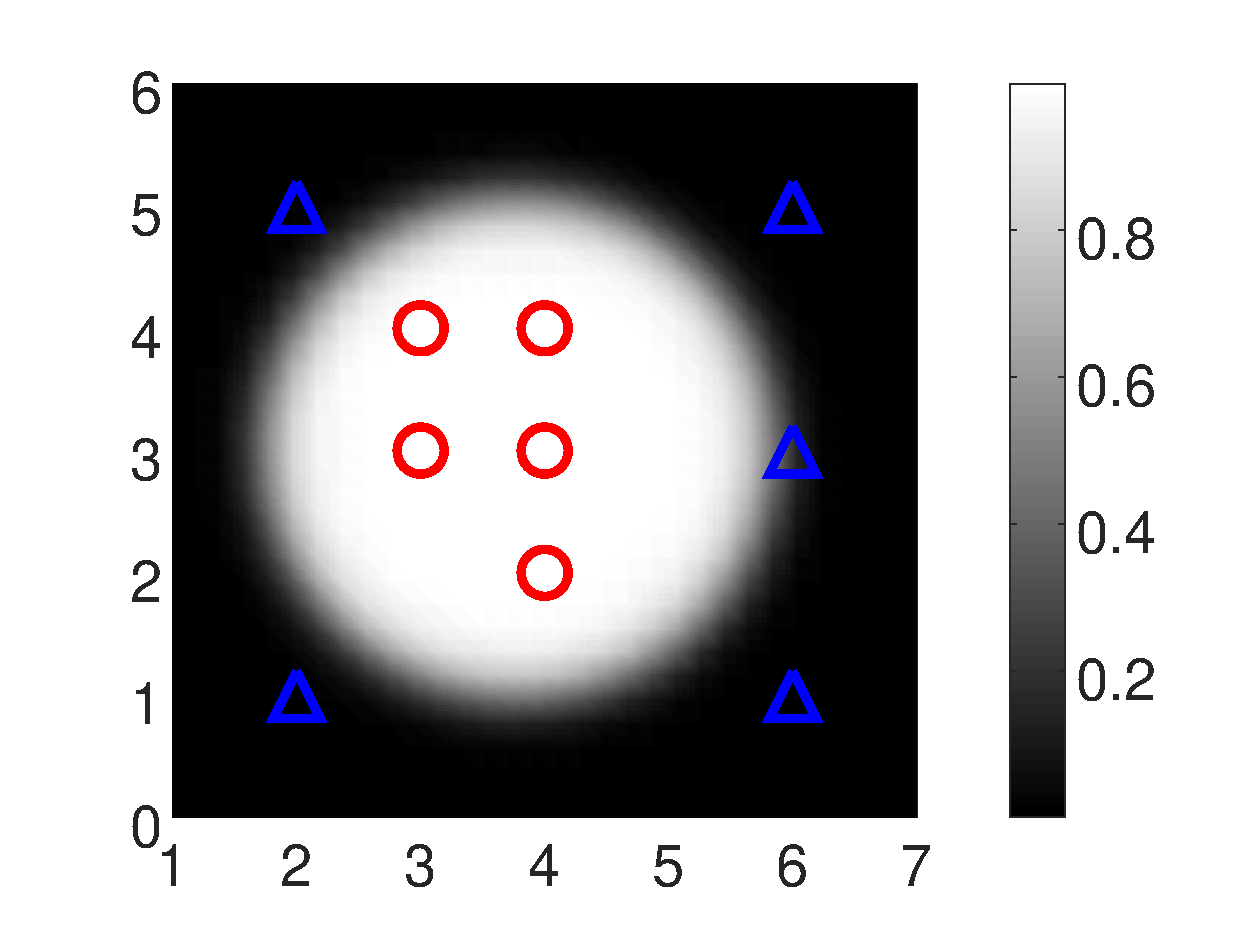
\includegraphics[width=0.45\textwidth]{chapters/classificacao/mfiles/reglogrnr1nolinear/ex1s2-reglogrnr1nolinear.eps}
        \caption{Gráfico da classificação usando $y_l \in \{0.001,~ 0.999\}$.}
        \label{fig:theo:reglogrnr1nolinear:xn:s1}
\end{figure}



